\chapter{Background Information}

Gait velocity estimation using pHRI depends two main components - modeling human walking and then using those models in an estimator. The models used in the estimator may be physics based or data-driven. Passive physics-based models such as the Bipedal Spring-Loaded Pendulum (B-SLIP) \cite{geyer2006compliant,liu2015dynamic} model are often used to model human locomotion. A passive model does not have any active control inputs to modify gaits and as steady-state human walking is periodic, optimization methods need to be used to find periodic model gaits. Poincar\'e maps are used in the gait optimization \cite{strogatz2018nonlinear,garcia1998simplest} to find periodic gaits.

\section{B-SLIP gaits}
\begin{figure}
	\centering
	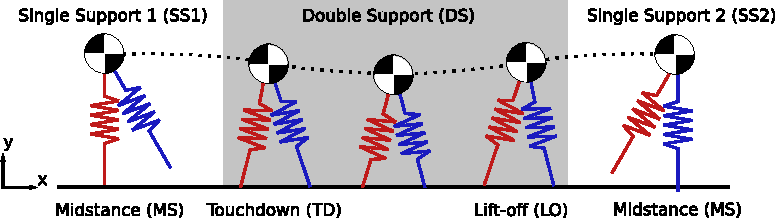
\includegraphics[width=0.9\linewidth]{slip_gait.pdf}
	\caption{One step of a B-SLIP gait}\label{fig:slip_gait}
\end{figure} 

A gait of the B-SLIP model is illustrated in Fig.~\ref{fig:slip_gait}. This gait is chosen to start at midstance (MS), where the CoM is loaded onto the trailing leg in single-support (SS1). The gait then proceeds with the touchdown (TD) of the leading leg and enters the double support (DS) phase. The DS phase ends with lift-off (LO) of the trailing leg and the model enters the second single-support phase (SS2). The SS2 phase ends in MS, again with the CoM loaded onto the leading leg.

\section{Poincar\'e maps}
\begin{figure}
	\centering
	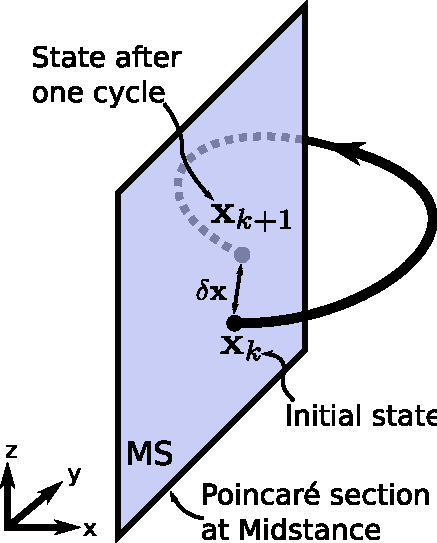
\includegraphics[width=.3\linewidth]{poincare.pdf}
	\caption{A Poincar\'e map used to find periodic gaits}\label{fig:poincare}
\end{figure}

A Poincar\'e section for a dynamical is a subspace that has fewer dimensions that the model's state space. It may be placed at a gait event such as MS, TD, or LO when the value of one of the states may be fixed e.g., when the vertical velocity of the \COM is zero. Let the Poincar\'e section be placed at MS, and let $ \mathcal{P} $ of the state $ \x_k $ be a function that returns the state after one cycle, or a step in the case of the B-SLIP, such that $ \x_{k+1} = \mathcal{P}(\x_k) $. The function $ \mathcal{P}(\x_k) $ is the Poincar\'e map and there exists an initial state representing a periodic orbit where the initial state maps back to itself after one period such that $ \x_k = \mathcal{P}(\x_k) $.
%
%\begin{equation}
%	\x_k = \mathcal{P}(\x_k)
%\end{equation}
%

A Poincar\'e section placed at MS is shown in blue in Fig.~\ref{fig:poincare}. The dynamics of the model are integrated for one step using $ \x_k $ as the initial condition. Optimization methods are used to find initial conditions that yield periodic gait by minimizing $ \delta \x $, the error between $ \x_k $ and $ \x_{k+1} $. The nonlinear return map may be linearized about these periodic gaits for further refining the gait search as described in Chapter \ref{chapter:IMM}. Model gaits for various velocities may be used as references while estimating an exoskeleton user's desired gait. Measurements of quantities such as CoM height and velocity, may be compared to simulated model gaits using state estimation tools such as the Kalman filter.

\section{State estimation using Kalman filters}

Kalman filtering is a feedback-based sequential optimal state estimation technique \cite{kalman1960new}. The optimality of this technique stems from the method of computing feedback gain that accounts for modeling and measurement errors. A fundamental assumption about the nature of these errors is that they are zero-mean Gaussian noise processes. The filter was originally proposed for discrete-time linear systems. 
 
The filter is initialized at a certain initial state estimate $ \hat{\x}_0 $ that may have associated uncertainty due to measurement errors. The evolution of this state is described using dynamical system presented in the following equations
%
\begin{eqnarray}
	\x_{k+1} &=& \A_k \x_k + \B_k \u_k + \mathbf{G} \mathbf{w}_k,\quad \mathbf{w}_k \sim \mathcal{N}(0, \Q_k) \label{eq:sys_disc}  \\
	\tilde{\y}_k &=& \H_k \x_k + \mathbf{v}_k,\quad \mathbf{v}_k \sim \mathcal{N}(0,\R_k) \label{eq:meas_lin}
\end{eqnarray}
%

\noindent where $ \x_k $ and $ \u_k $ are the discrete-time states and inputs, $ \y_k $ are the discrete-time measurements, $ \A_k $, $ \B_k $, $ \H_k $ are the system, input, and measurement models respectively. The system has zero-mean Gaussian noises for process noise $ \mathbf{w}_k $ and measurement noise $ \mathbf{v}_k $ with covariances  $ \Q_k $ and $ \R_k $ respectively. The measurement noise $ \mathbf{w}(t) $ is combined with the measurement equation $ \H_k \x_k$ to form the noisy measurement $ \tilde{\y}_k $. 

\begin{figure}
	\centering
	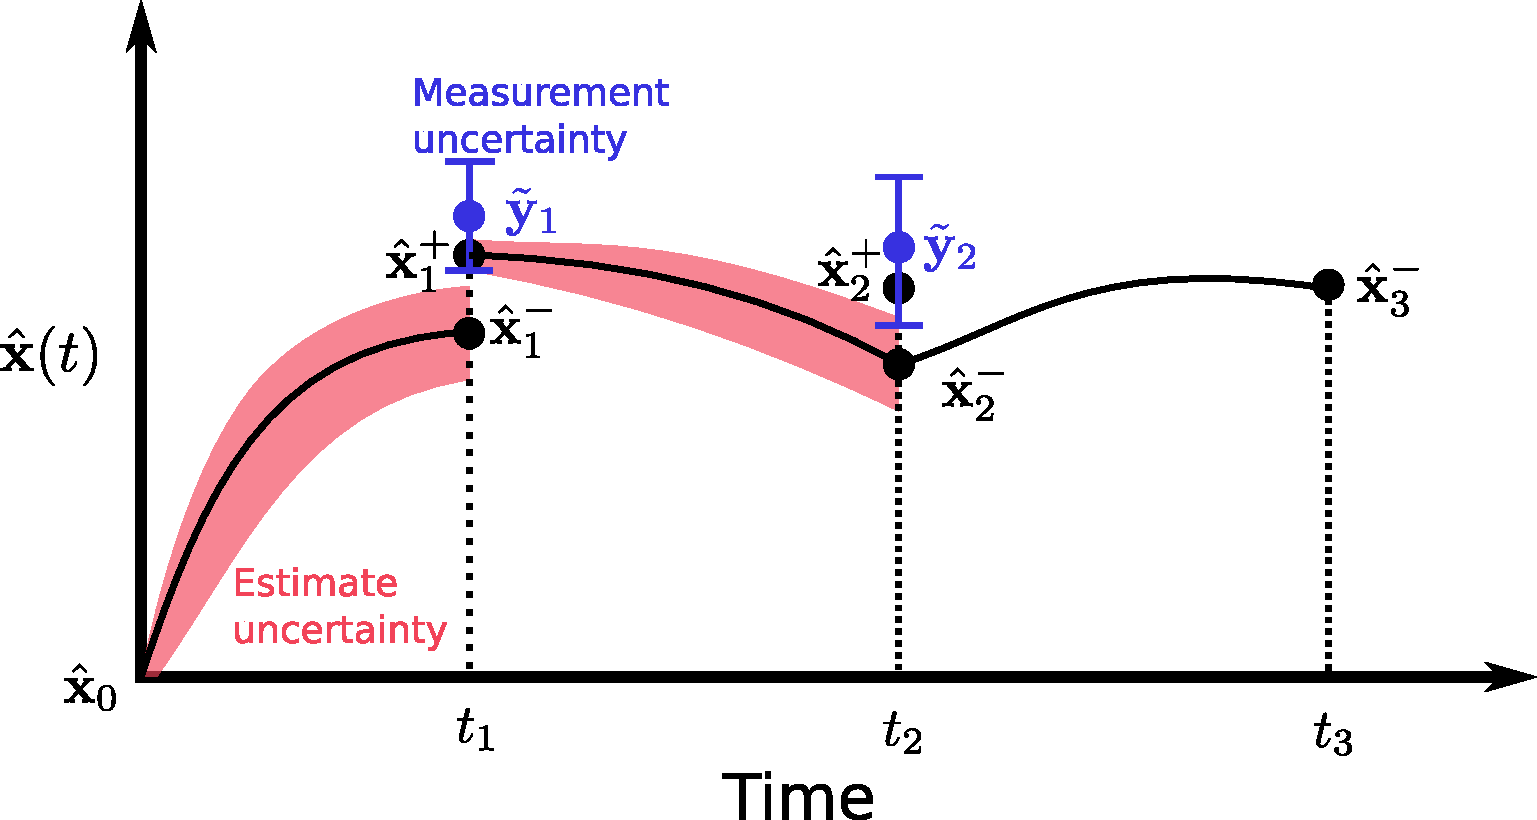
\includegraphics[width=0.7\linewidth]{kalman.pdf}
	\caption{Illustration of the Kalman Filtering process}\label{fig:kalman}
\end{figure}

The uncertainty associated with the estimates increases as the state is propagated forward through time using the system dynamics. Regular measurements of state variables are used to update the state estimates and reduce the uncertainty as illustrated in Fig.~\ref{fig:kalman} where the $ + $ and $ - $ in the superscript denote pre- and post-update states. The system illustrated here is discrete, however a continuous state evolution is shown to better illustrate the growth in uncertainty. Kalman filters account for both, the uncertainty in the state estimates and in the measurements. Further details of this process are as follow. The state estimates and estimate covariance $ \P $ are propagated in discrete time such that
\begin{eqnarray}
	\hat{\x}_{k+1} &=& \A_k \hat{\x}_k + \B_k \u_k \\
	\P_{k+1} &=& \A_k\P_k \A_k^T + \mathbf{G}_k\Q_k\mathbf{G}_k^T 
\end{eqnarray}
\noindent The states are sequentially updated such that
\begin{eqnarray}
	\K_k &=& \P_k^- \H^T_k \left[\H_k \P_k^- \H^T_k + \R_k\right]^{-1} \\
	\hat{\x}_k^+ &=& \hat{\x}_k^- + \K_k[\tilde{\y}_k- \H_k \hat{\x}_k^-)] \\
	\P_k^+ &=& [\mathbf{I} - \K_k \H_k]\P_k^-
\end{eqnarray}

\noindent where the updated estimates, their covariance and the Kalman gain are $ \mathbf{x}_k^+ $, $ \mathbf{P}_k^+ $, and $ \K_k $ respectively. The Kalman gain is optimal and the error dynamics of the filter are shown to be stable \cite{Crassidis} using the Lyapunov candidate function $ V(\e) = \e_k^T P_k^{-1} \e_k $ where $ \e_k \equiv \hat{\x}_k - \x_k $. The filter as described above is defined for linear systems, and it has been extended to nonlinear systems.

Simple models used to describe legged locomotion have nonlinear dynamics and a variation of the Kalman filter named the Extended Kalman Filter (EKF) can be used for these systems. The nonlinear dynamics are linearized about the state estimate to work around the nonlinearity. As this linearization is an approximation of the dynamics, the EKF is not optimal like the discrete-time Kalman filter described previously. In spite of the lack of optimality, EKFs have been in widespread use for nonlinear systems. Since most nonlinear dynamics are given in continuous time, a variation of the EKF called the Continuous-Discrete EKF may be used. In this variation, dynamics evolve in continuous time, and measurements are modeled in discrete time. This combination is used for estimation in the work presented herein as it most closely reflects the model and measurement conditions observed in the estimation problem being studied. Consider the following dynamical system
% Continuous-Discrete EKF
%
\begin{eqnarray}
	\dot{\x}(t) &=& \mathbf{f}(\x(t),\u(t),\mathbf{w}(t),t),\quad \mathbf{w}(t) \sim \mathcal{N}(0, \Q(t))  \label{eq:sys}  \\
	\tilde{\y}_k &=& \mathbf{h}(\x_k) + \mathbf{v}_k,\quad \mathbf{v}_k \sim \mathcal{N}(0,\R_k) \label{eq:meas}
\end{eqnarray}
%
\noindent where $ \x(t) $ and $ \u(t) $ are the continuous-time states and inputs, $ \y_k $ are the discrete-time measurements, and $ \mathbf{f}(\x(t),\u(t),t) $ and $ \mathbf{h}(\x_k) $ are the system and measurement function respectively. The system has zero-mean Gaussian process and measurement noises $ \mathbf{w}(t) $ and $ \mathbf{v}_k $ respectively with covariances $ \Q(t) $ and $ \R_k $ respectively. The measurement noise $ \mathbf{w}(t) $ is combined with the measurement equation $ \mathbf{h}(\x_k) $ to form the noisy measurement $ \tilde{\y}_k $. 

The state estimates and estimate covariance $ \P $ are propagated in continuous time such that
\begin{eqnarray}
	\dot{\hat{\x}} &=& \mathbf{f}(\hat{\x},\u,t) \\
	\dot{\P}(t) &=& \F(t)\P(t) + \P(t)\F^T(t) + \mathbf{G}(t)\Q(t)\mathbf{G}(t)^T \\ 
	\F(t) &\equiv& \frac{\partial \mathbf{f}}{\partial \x} \Bigr |_{\hat{\x}(t),\u(t)} \nonumber
\end{eqnarray}


\noindent The states are sequentially updated such that
\begin{eqnarray}
	\K_k &=& \P_k^- \H^T_k(\hat{\x}_k^-) \left[\H_k(\hat{\x}_k^-)\P_k^- \H^T_k(\hat{\x}_k^-) + \R_k\right]^{-1} \\
	\hat{\x}_k^+ &=& \hat{\x}_k^- + \K_k[\tilde{\y}_k-\mathbf{h}(\x_k)] \\
	\P_k^+ &=& [\mathbf{I} - \K_k \H_k(\hat{\x}_k^-)]\P_k^-,\quad \H_k(\hat{\x}_k^-) \equiv \frac{\partial \mathbf{h}}{\partial \x} \Bigr |_{\hat{\x}_k^-}
\end{eqnarray}

\noindent where $ \K_k $ is the Kalman gain, $ \F(t) $, and $ \H_k(\hat{\x}_k^-) $ are the linearized dynamics and measurement model respectively. The updated estimates and their covariance are $ \mathbf{x}_k^+ $ and $ \mathbf{P}_k^+ $ respectively. The above equations describe a Continous-Discrete Kalman filter setup. System dynamics are propagated in continuous time but states are updated in discrete time since measurements are discrete. This setup handles the nonlinear dynamics of the models used to emulate legged locomotion. Each step of human walking has alternating single and double support periods depending on how many legs are in contact with the ground. Therefore, addition to being nonlinear, models of legged locomotion have hybrid dynamics to describe different gait phases i.e., different dynamics for different phases. The EKF can be used as an estimation tool to handle these hybrid dynamics in a framework known as Interacting Multi-Model (IMM) estimation. This framework is used in Chapter~\ref{chapter:IMM} to estimate an exoskeleton user's gait speed and gait phase.